\documentclass{beamer}
\usepackage[english,russian]{babel}
\usepackage[utf8]{inputenc}
\usepackage{amsmath}
\usepackage{hyperref}
\usetheme{Warsaw}
\usepackage{listings}
\usepackage{xcolor}
\usepackage{tikz}
\usetikzlibrary{graphs}

\lstset{
    frame=tb,
    tabsize=4,
    showstringspaces=false,
    numbers=left,
    commentstyle=\color{green},
    keywordstyle=\color{blue},
    stringstyle=\color{red},
    emph={baz},
    emphstyle=\textbf
}

\begin{document}

\title{Задачи разрешимости логических формул и приложения\newline Лекция 2. SAT задача. Сведение задачи к SAT задаче}
\author{Роман Холин}
\institute{Московский государственный университет}
\date{Москва, 2021}

\begin{frame}
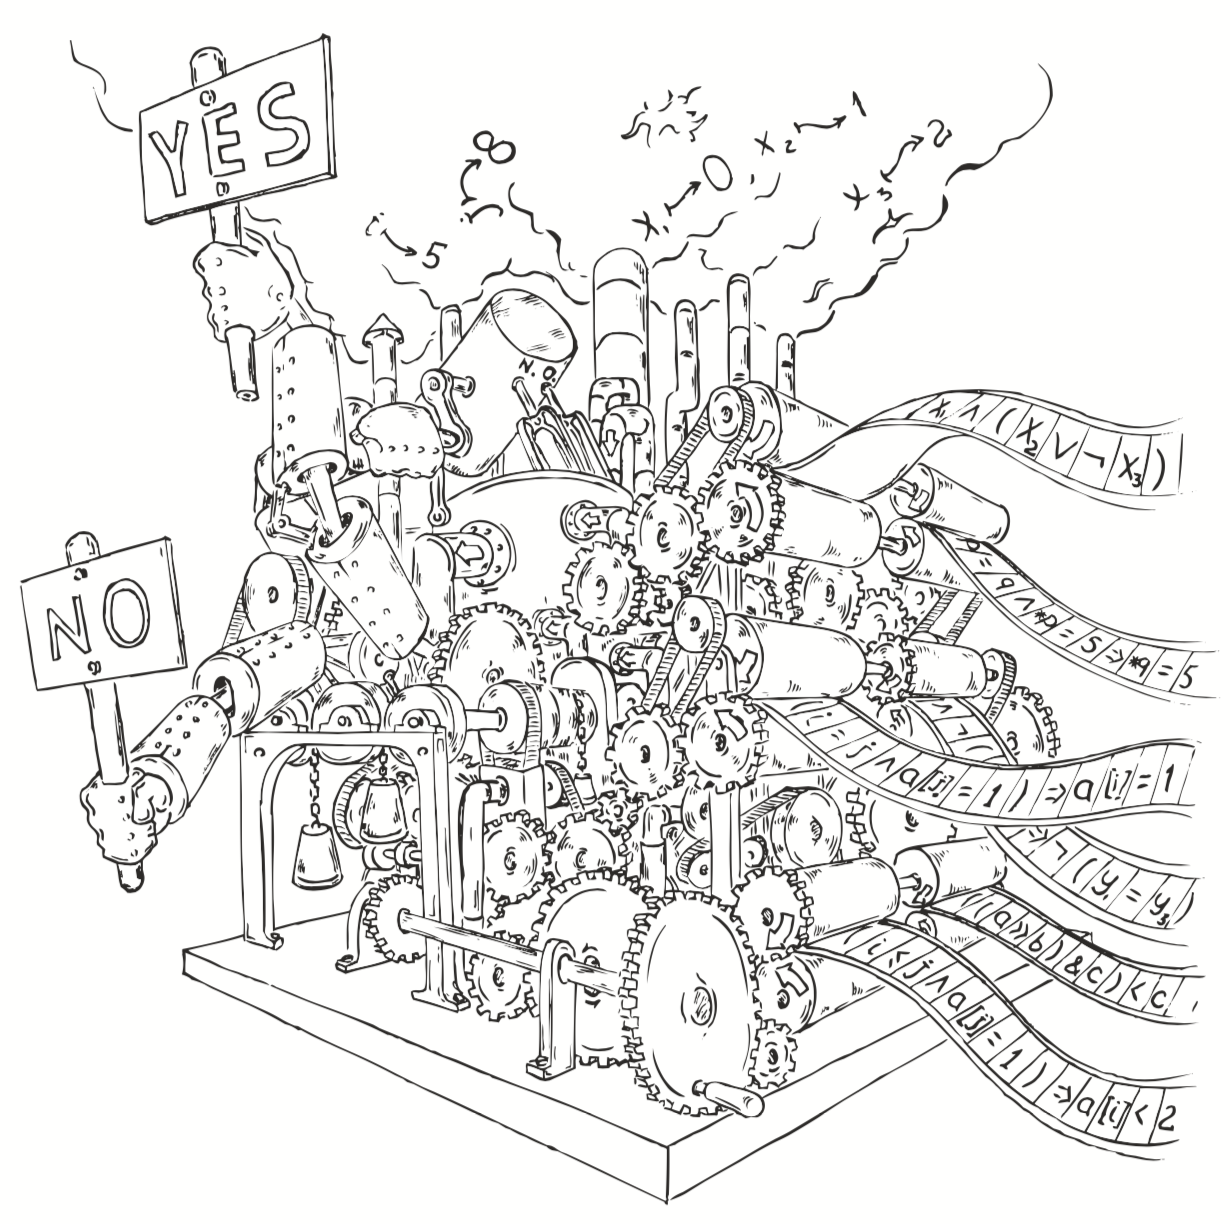
\includegraphics[scale=0.5]{../decision-procedure.png}
\end{frame}

\frame{\titlepage}

\begin{frame}{Дополнительные материалы}
\begin{itemize}
\item Decision Procedures An Algorithmic Point of View, Daniel Kroening, Ofer Strichman
\item Handbook of satisfiability, Edmund Clarke
\item The art of Computer Programming, volume 4, part 6, Donald Knuth
\end{itemize}
\end{frame}

\begin{frame}{Дополнительные материалы}
\begin{itemize}
\item \href{http://composition.al/CSE290Q-2019-09/index.html}{cse290q}
\item \href{https://courses.cs.washington.edu/courses/cse507/19au/calendar.html}{cse507}
\item \href{https://www.cs.cmu.edu/~mheule/15816-f19/schedule.html}{15816-f19}
\end{itemize}
\end{frame}

\begin{frame}{AtLeastOne}
\begin{itemize}
\item Рассмотрим функцию $AtLeastOne(x_1, \dots, x_n)$ - истина ли хотя бы одна из переменных
\end{itemize}
\end{frame}

\begin{frame}{AtLeastOne}
\begin{itemize}
\item Рассмотрим функцию $AtLeastOne(x_1, \dots, x_n)$ - истина ли хотя бы одна из переменных
\item Как её выразить в КНФ?
\end{itemize}
\end{frame}

\begin{frame}{AtLeastOne}
\begin{itemize}
\item Рассмотрим функцию $AtLeastOne(x_1, \dots, x_n)$ - истина ли хотя бы одна из переменных
\item Как её выразить в КНФ?
\item $(x_1 \vee \dots \vee x_n)$
\end{itemize}
\end{frame}

\begin{frame}{XOR}
\begin{itemize}
\item Аналогичный вопрос про $XOR(x_1, \dots, x_n)$
\end{itemize}
\end{frame}

\begin{frame}{XOR}
\begin{itemize}
\item Аналогичный вопрос про $XOR(x_1, \dots, x_n)$
\item Пусть $x^{\alpha} = (x \leftrightarrow \alpha)$
\item $XOR = \bigwedge(x_1^{\alpha_1} \vee \dots \vee x_n^{\alpha_n})$, т.е. $\wedge$ по всем наборам $\alpha$, таким,
$\Sigma_i(\alpha_i)$ - четное число.
\end{itemize}
\end{frame}

\begin{frame}{XOR}
\begin{itemize}
\item Аналогичный вопрос про $XOR(x_1, \dots, x_n)$
\item Пусть $x^{\alpha} = (x \leftrightarrow \alpha)$
\item $XOR = \bigwedge(x_1^{\alpha_1} \vee \dots \vee x_n^{\alpha_n})$, т.е. $\wedge$ по всем наборам $\alpha$, таким,
$\Sigma_i(\alpha_i)$ - четное число.
\item Сколько дизъюнктов в такой формуле? Можно ли сделать меньше?
\end{itemize}
\end{frame}

\begin{frame}{XOR}
\begin{itemize}
\item Аналогичный вопрос про $XOR(x_1, \dots, x_n)$
\item Пусть $x^{\alpha} = (x \leftrightarrow \alpha)$
\item $XOR = \bigwedge(x_1^{\alpha_1} \vee \dots \vee x_n^{\alpha_n})$, т.е. $\wedge$ по всем наборам $\alpha$, таким,
$\Sigma_i(\alpha_i)$ - четное число.
\item Сколько дизъюнктов в такой формуле? Можно ли сделать меньше?
\item $XOR(x_1, x_2, y) \wedge XOR(\lnot y, x_3, \dots, x_n)$
\end{itemize}
\end{frame}

\begin{frame}{AtMostOne}
\begin{itemize}
\item $AtMostOne(x_1, \dots, x_n)$ - истина, если среди $x_1, \dots, x_n$ не более одной истиной переменной.
\end{itemize}
\end{frame}

\begin{frame}{AtMostOne}
\begin{itemize}
\item $AtMostOne(x_1, \dots, x_n)$ - истина, если среди $x_1, \dots, x_n$ не более одной истиной переменной.
\item \[\bigwedge_{1 \le i < j \le n}(\lnot x_i \vee \lnot x_j)\]
\end{itemize}
\end{frame}

\begin{frame}{AtMostOne}
\begin{itemize}
\item $AtMostOne(x_1, \dots, x_n)$ - истина, если среди $x_1, \dots, x_n$ не более одной истиной переменной.
\item \[\bigwedge_{1 \le i < j \le n}(\lnot x_i \vee \lnot x_j)\]
\item Сколько дизъюнктов в такой формуле? Можно ли сделать меньше?
\end{itemize}
\end{frame}

\begin{frame}{AtMostOne}
\begin{itemize}
\item $AtMostOne(x_1, \dots, x_n)$ - истина, если среди $x_1, \dots, x_n$ не более одной истиной переменной.
\item \[\bigwedge_{1 \le i < j \le n}(\lnot x_i \vee \lnot x_j)\]
\item Сколько дизъюнктов в такой формуле? Можно ли сделать меньше?
\item $AtMostOne(x_1, x_2, x_3, y) \vee AtMostOne(\lnot y, x_4, \dots, x_n)$
\end{itemize}
\end{frame}

\begin{frame}{AtMostOne}
\begin{itemize}
\item $AtMostOne(x_1, x_2)$:\newline
\end{itemize}
\end{frame}

\begin{frame}{AtMostOne}
\begin{itemize}
\item $AtMostOne(x_1, x_2)$:\newline
$\phi_1 = \lnot x_1 \vee \lnot x_2$\newline
$\phi_2 = (\lnot x_1 \vee y) \wedge (y \lnot x_2)$\newline
\end{itemize}
\end{frame}

\begin{frame}{AtMostOne}
\begin{itemize}
\item $AtMostOne(x_1, x_2)$:\newline
$\phi_1 = \lnot x_1 \vee \lnot x_2$\newline
$\phi_2 = (\lnot x_1 \vee y) \wedge (y \lnot x_2)$\newline
\item Они эквивалентны?
\end{itemize}
\end{frame}

\begin{frame}{AtMostOne}
\begin{itemize}
\item $AtMostOne(x_1, x_2)$:\newline
$\phi_1 = \lnot x_1 \vee \lnot x_2$\newline
$\phi_2 = (\lnot x_1 \vee y) \wedge (y \lnot x_2)$\newline
\item Они эквивалентны?
\item $\phi_1 \leftrightarrow \phi_2$ - тавтология, если и $\lnot \phi_1 \wedge \phi_2$ и $\phi_1 \wedge \lnot \phi_2$ -
невыполнима.
\end{itemize}
\end{frame}

\begin{frame}{AtMostOne}
\begin{itemize}
\item $AtMostOne(x_1, x_2)$:\newline
$\phi_1 = \lnot x_1 \vee \lnot x_2$\newline
$\phi_2 = (\lnot x_1 \vee y) \wedge (y \lnot x_2)$\newline
\item Они эквивалентны?
\item $\phi_1 \leftrightarrow \phi_2$ - тавтология, если и $\lnot \phi_1 \wedge \phi_2$ и $\phi_1 \wedge \lnot \phi_2$ -
невыполнима.
\item Выполнима ли $\lnot \phi_1 \wedge \phi_2$?
\end{itemize}
\end{frame}

\begin{frame}{AtMostOne}
\begin{itemize}
\item $AtMostOne(x_1, x_2)$:\newline
$\phi_1 = \lnot x_1 \vee \lnot x_2$\newline
$\phi_2 = (\lnot x_1 \vee y) \wedge (y \lnot x_2)$\newline
\item Они эквивалентны?
\item $\phi_1 \leftrightarrow \phi_2$ - тавтология, если и $\lnot \phi_1 \wedge \phi_2$ и $\phi_1 \wedge \lnot \phi_2$ -
невыполнима.
\item Выполнима ли $\lnot \phi_1 \wedge \phi_2$?
\item Выполнима ли $\phi_1 \wedge \lnot \phi_2$?
\end{itemize}
\end{frame}

\begin{frame}{AtMostOne}
\begin{itemize}
\item $AtMostOne(x_1, x_2)$:\newline
$\phi_1 = \lnot x_1 \vee \lnot x_2$\newline
$\phi_2 = (\lnot x_1 \vee y) \wedge (y \lnot x_2)$\newline
\item Они эквивалентны?
\item $\phi_1 \leftrightarrow \phi_2$ - тавтология, если и $\lnot \phi_1 \wedge \phi_2$ и $\phi_1 \wedge \lnot \phi_2$ -
невыполнима.
\item Выполнима ли $\lnot \phi_1 \wedge \phi_2$?
\item Выполнима ли $\phi_1 \wedge \lnot \phi_2$?
\item Формулы не эквивалентны, но равносильны, т.е. $\phi_1$ - выполнима, тогда и только тогда, когда $\phi_2$ - выполнима.
\end{itemize}
\end{frame}

\begin{frame}{Преобразование булевой формулы в КНФ}
\begin{itemize}
\item Какова сложность преобразование формулы в КНФ?
\end{itemize}
\end{frame}

\begin{frame}{Преобразование булевой формулы в КНФ}
\begin{itemize}
\item Какова сложность преобразование формулы в КНФ?
\item В худшем случае экспонента
\end{itemize}
\end{frame}

\begin{frame}{Преобразование булевой формулы в КНФ}
\begin{itemize}
\item Какова сложность преобразование формулы в КНФ?
\item В худшем случае экспонента
\item Например $(x_1 \wedge y_1) \vee \dots \vee (x_n \wedge y_n)$, преобразовывая с помощью законов Де Моргана и закона
дистрибутивности к формуле $(x_1 \vee \dots \vee x_n) \wedge (y_1 \vee x_2 \vee \dots \vee x_n) \wedge (y_1 \vee \dots \vee y_n)$
- получаем $2^n$ дизъюнктов.
\end{itemize}
\end{frame}

\begin{frame}{Преобразование Цейтина (Tseytin transformation)}
\begin{itemize}
\item $P \rightarrow (Q \wedge R)$
\end{itemize}
\end{frame}

\begin{frame}{Преобразование Цейтина (Tseytin transformation)}
\begin{itemize}
\item $P \rightarrow (Q \wedge R)$
\item Введем переменные для всех неатомарных подформул:\newline
$T_1 \leftrightarrow P \rightarrow T_2$\newline
$T_2 \leftrightarrow (Q \wedge R)$\newline
\end{itemize}
\end{frame}

\begin{frame}{Преобразование Цейтина (Tseytin transformation)}
\begin{itemize}
\item $P \rightarrow (Q \wedge R)$
\item Введем переменные для всех неатомарных подформул:\newline
$T_1 \leftrightarrow P \rightarrow T_2$\newline
$T_2 \leftrightarrow (Q \wedge R)$\newline
\item Каждую преобразуем в КНФ:\newline
$F_1 = (T_1 \vee P) \wedge (T_1 \vee \lnot T_2) \wedge (\lnot T_1 \vee \lnot P \vee T_2)$\newline
$F_2 = (\lnot T_2 \vee Q) \wedge (\lnot T_2 \vee R) \wedge (T_2 \vee \lnot Q \vee \lnot R)$\newline
\end{itemize}
\end{frame}

\begin{frame}{Преобразование Цейтина (Tseytin transformation)}
\begin{itemize}
\item $P \rightarrow (Q \wedge R)$
\item Введем переменные для всех неатомарных подформул:\newline
$T_1 \leftrightarrow P \rightarrow T_2$\newline
$T_2 \leftrightarrow (Q \wedge R)$\newline
\item Каждую преобразуем в КНФ:\newline
$F_1 = (T_1 \vee P) \wedge (T_1 \vee \lnot T_2) \wedge (\lnot T_1 \vee \lnot P \vee T_2)$\newline
$F_2 = (\lnot T_2 \vee Q) \wedge (\lnot T_2 \vee R) \wedge (T_2 \vee \lnot Q \vee \lnot R)$\newline
\item $T_1 \wedge F_1 \wedge F_2$
\end{itemize}
\end{frame}

\begin{frame}{Гамильтонов цикл}
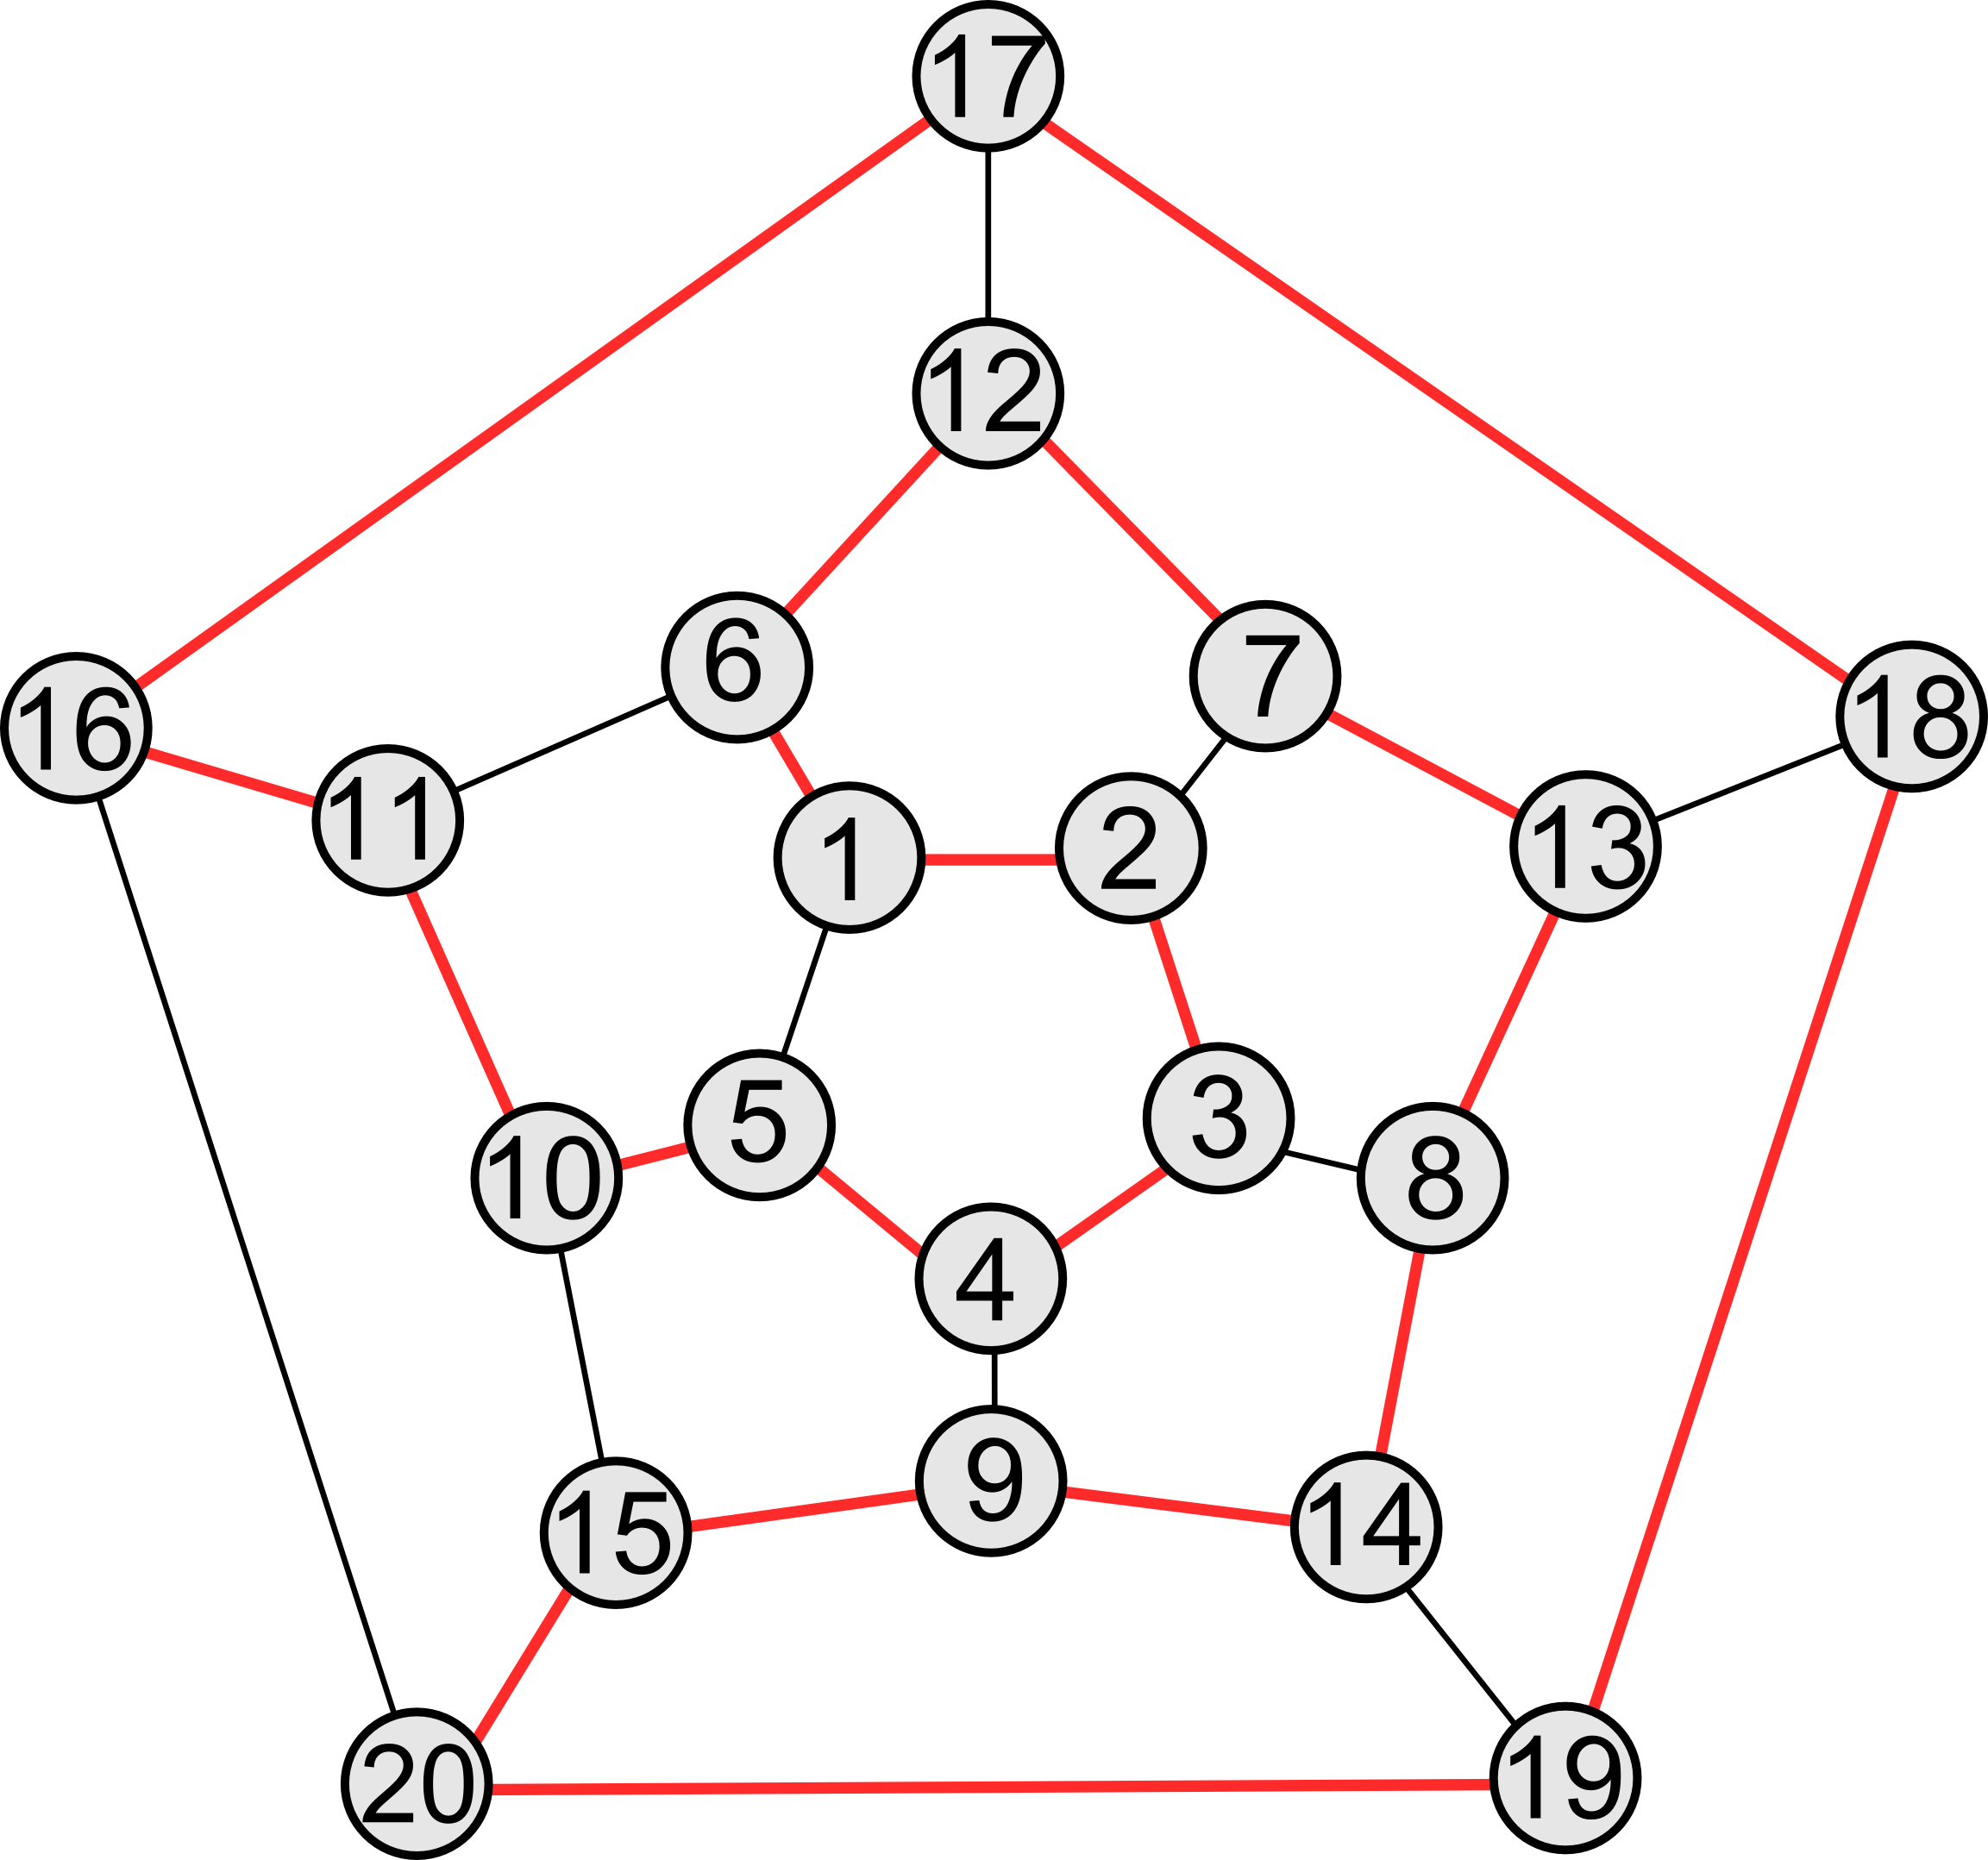
\includegraphics[scale=0.4]{Hamiltonial.png}
\end{frame}

\begin{frame}{Гамильтонов цикл}
\begin{itemize}
\item $\Sigma_{j} x_{ij} = 1$ - для каждого $i$ (т.е. для всех исходящих ребер)
\end{itemize}
\end{frame}

\begin{frame}{Гамильтонов цикл}
\begin{itemize}
\item $\Sigma_{j} x_{ij} = 1$ - для каждого $i$ (т.е. для всех исходящих ребер)
\item $\Sigma_{i} x_{ij} = 1$ - для каждого $j$ (т.е. для всех входящих ребер)
\end{itemize}
\end{frame}

\begin{frame}{Гамильтонов цикл}
\begin{itemize}
\item $\Sigma_{j} x_{ij} = 1$ - для каждого $i$ (т.е. для всех исходящих ребер)
\item $\Sigma_{i} x_{ij} = 1$ - для каждого $j$ (т.е. для всех входящих ребер)
\item $\Sigma_{ij \in S} x_{ij} \le |S| - 1$, где $S$ - подмножество V и $2 \le |S| \le n - 2$ - связность графа
\end{itemize}
\end{frame}

\begin{frame}{Гамильтонов цикл}
\begin{itemize}
\item Проблема - очень много ограничений.
\item Только добавление всех троек дает $O(n^3)$ уравнений.
\end{itemize}
\end{frame}

\begin{frame}{Гамильтонов цикл}
\begin{itemize}
\item Проблема - очень много ограничений.
\item Только добавление всех троек дает $O(n^3)$ уравнений.
\item Давайте поступать лениво!
\item Пусть сначало в нашей системе урванений нет ограничений на связанность
\item Попросим солвер решить нашу систему. Если в ответе получился путь, в котором не все ребра есть в графе, то добавим в
систему уравнений ограничение на текущий путь.
\end{itemize}
\end{frame}

\begin{frame}{Гамильтонов цикл}
\begin{itemize}
\item Проблема - очень много ограничений.
\item Только добавление всех троек дает $O(n^3)$ уравнений.
\item Давайте поступать лениво!
\item Пусть сначало в нашей системе урванений нет ограничений на связанность
\item Попросим солвер решить нашу систему. Если в ответе получился путь, в котором не все ребра есть в графе, то добавим в
систему уравнений ограничение на текущий путь.
\item Практика показывает, что хватит $O(n^3)$ дополнительных уравнений.
\end{itemize}
\end{frame}

\begin{frame}{DIMACS формат}
\begin{itemize}
\item Комментарий c comment
\item Заголовок p cnf n m: n - количество переменных в дизюнкте, m - количество дизюнктов
\item Дизъюнкт - описание дизъюнкта: номера переменных, который в него входят, <<->> - если переменная ложная, в конце всегда 0
\end{itemize}
\end{frame}

\begin{frame}{DIMACS формат}
\begin{itemize}
\item Комментарий c comment
\item Заголовок p cnf n m: n - количество переменных в дизюнкте, m - количество дизюнктов
\item Дизъюнкт - описание дизъюнкта: номера переменных, который в него входят, <<->> - если переменная ложная, в конце всегда 0
\item $(a \vee b \vee \lnot c) \wedge (\lnot a \vee \lnot b \vee c) \wedge (b \vee c \vee \lnot d)$
\item c example\newline
p cnf 4 7\newline
1 2 -3 0\newline
-1 -2 3 0\newline
2 3 -4 0\newline
\end{itemize}
\end{frame}

\begin{frame}
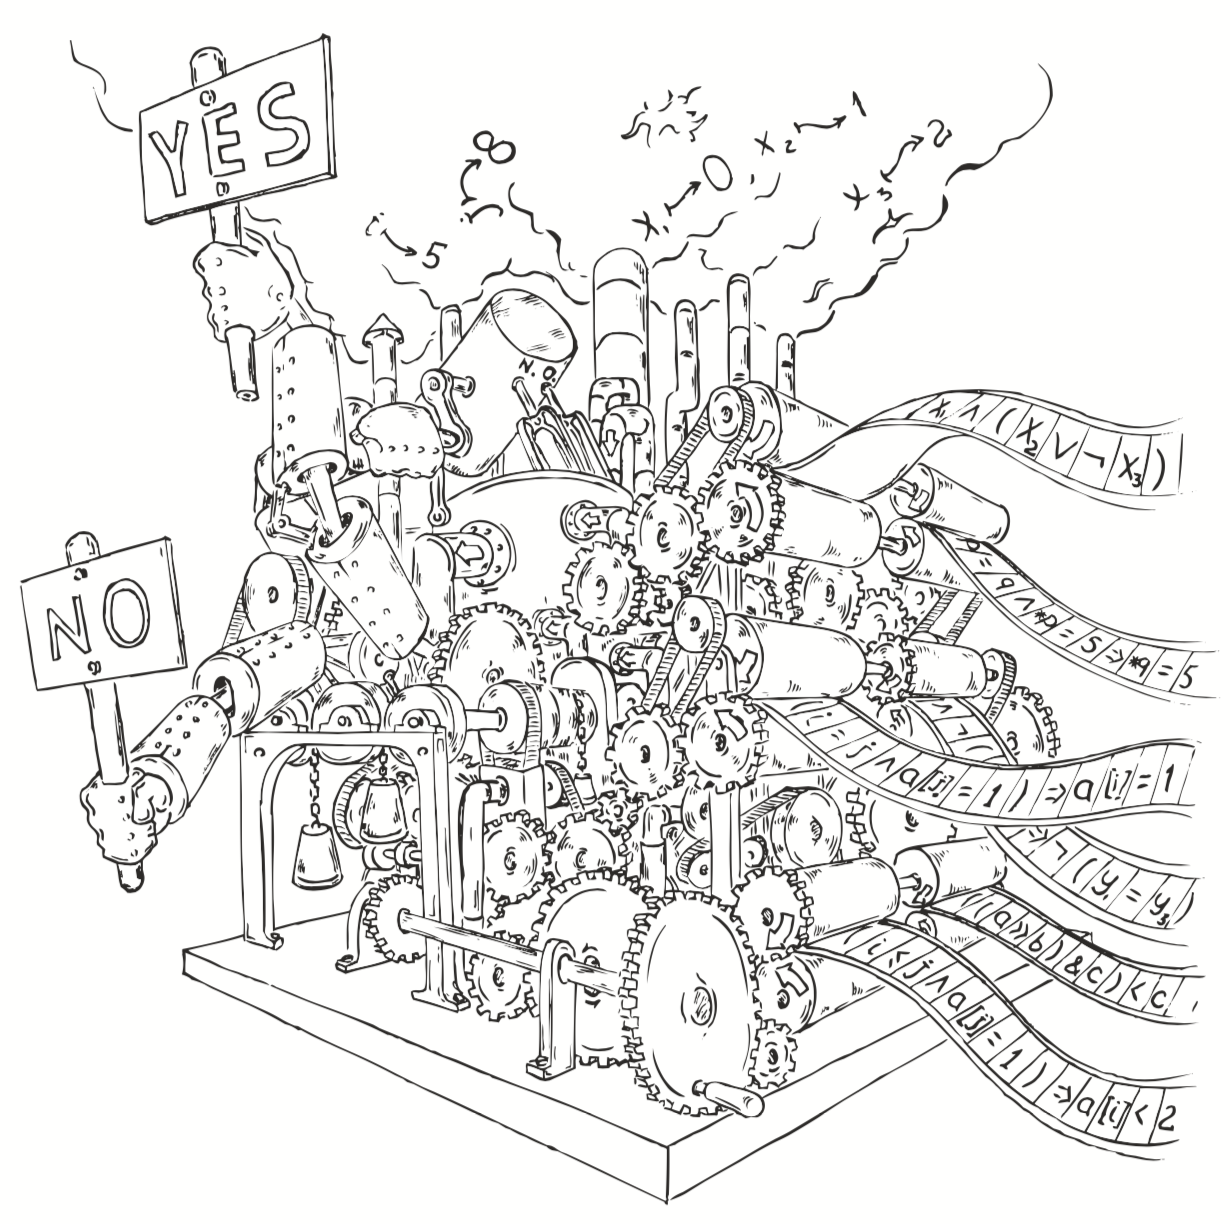
\includegraphics[scale=0.5]{../decision-procedure.png}
\end{frame}

\end{document}
